\documentclass[1p]{elsarticle_modified}
%\bibliographystyle{elsarticle-num}

%\usepackage[colorlinks]{hyperref}
%\usepackage{abbrmath_seonhwa} %\Abb, \Ascr, \Acal ,\Abf, \Afrak
\usepackage{amsfonts}
\usepackage{amssymb}
\usepackage{amsmath}
\usepackage{amsthm}
\usepackage{scalefnt}
\usepackage{amsbsy}
\usepackage{kotex}
\usepackage{caption}
\usepackage{subfig}
\usepackage{color}
\usepackage{graphicx}
\usepackage{xcolor} %% white, black, red, green, blue, cyan, magenta, yellow
\usepackage{float}
\usepackage{setspace}
\usepackage{hyperref}

\usepackage{tikz}
\usetikzlibrary{arrows}

\usepackage{multirow}
\usepackage{array} % fixed length table
\usepackage{hhline}

%%%%%%%%%%%%%%%%%%%%%
\makeatletter
\renewcommand*\env@matrix[1][\arraystretch]{%
	\edef\arraystretch{#1}%
	\hskip -\arraycolsep
	\let\@ifnextchar\new@ifnextchar
	\array{*\c@MaxMatrixCols c}}
\makeatother %https://tex.stackexchange.com/questions/14071/how-can-i-increase-the-line-spacing-in-a-matrix
%%%%%%%%%%%%%%%

\usepackage[normalem]{ulem}

\newcommand{\msout}[1]{\ifmmode\text{\sout{\ensuremath{#1}}}\else\sout{#1}\fi}
%SOURCE: \msout is \stkout macro in https://tex.stackexchange.com/questions/20609/strikeout-in-math-mode

\newcommand{\cancel}[1]{
	\ifmmode
	{\color{red}\msout{#1}}
	\else
	{\color{red}\sout{#1}}
	\fi
}

\newcommand{\add}[1]{
	{\color{blue}\uwave{#1}}
}

\newcommand{\replace}[2]{
	\ifmmode
	{\color{red}\msout{#1}}{\color{blue}\uwave{#2}}
	\else
	{\color{red}\sout{#1}}{\color{blue}\uwave{#2}}
	\fi
}

\newcommand{\Sol}{\mathcal{S}} %segment
\newcommand{\D}{D} %diagram
\newcommand{\A}{\mathcal{A}} %arc


%%%%%%%%%%%%%%%%%%%%%%%%%%%%%5 test

\def\sl{\operatorname{\textup{SL}}(2,\Cbb)}
\def\psl{\operatorname{\textup{PSL}}(2,\Cbb)}
\def\quan{\mkern 1mu \triangleright \mkern 1mu}

\theoremstyle{definition}
\newtheorem{thm}{Theorem}[section]
\newtheorem{prop}[thm]{Proposition}
\newtheorem{lem}[thm]{Lemma}
\newtheorem{ques}[thm]{Question}
\newtheorem{cor}[thm]{Corollary}
\newtheorem{defn}[thm]{Definition}
\newtheorem{exam}[thm]{Example}
\newtheorem{rmk}[thm]{Remark}
\newtheorem{alg}[thm]{Algorithm}

\newcommand{\I}{\sqrt{-1}}
\begin{document}

%\begin{frontmatter}
%
%\title{Boundary parabolic representations of knots up to 8 crossings}
%
%%% Group authors per affiliation:
%\author{Yunhi Cho} 
%\address{Department of Mathematics, University of Seoul, Seoul, Korea}
%\ead{yhcho@uos.ac.kr}
%
%
%\author{Seonhwa Kim} %\fnref{s_kim}}
%\address{Center for Geometry and Physics, Institute for Basic Science, Pohang, 37673, Korea}
%\ead{ryeona17@ibs.re.kr}
%
%\author{Hyuk Kim}
%\address{Department of Mathematical Sciences, Seoul National University, Seoul 08826, Korea}
%\ead{hyukkim@snu.ac.kr}
%
%\author{Seokbeom Yoon}
%\address{Department of Mathematical Sciences, Seoul National University, Seoul, 08826,  Korea}
%\ead{sbyoon15@snu.ac.kr}
%
%\begin{abstract}
%We find all boundary parabolic representation of knots up to 8 crossings.
%
%\end{abstract}
%\begin{keyword}
%    \MSC[2010] 57M25 
%\end{keyword}
%
%\end{frontmatter}

%\linenumbers
%\tableofcontents
%
\newcommand\colored[1]{\textcolor{white}{\rule[-0.35ex]{0.8em}{1.4ex}}\kern-0.8em\color{red} #1}%
%\newcommand\colored[1]{\textcolor{white}{ #1}\kern-2.17ex	\textcolor{white}{ #1}\kern-1.81ex	\textcolor{white}{ #1}\kern-2.15ex\color{red}#1	}

{\Large $\underline{12a_{1249}~(K12a_{1249})}$}

\setlength{\tabcolsep}{10pt}
\renewcommand{\arraystretch}{1.6}
\vspace{1cm}\begin{tabular}{m{100pt}>{\centering\arraybackslash}m{274pt}}
\multirow{5}{120pt}{
	\centering
	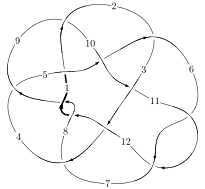
\includegraphics[width=112pt]{../../../GIT/diagram.site/Diagrams/png/2050_12a_1249.png}\\
\ \ \ A knot diagram\footnotemark}&
\allowdisplaybreaks
\textbf{Linearized knot diagam} \\
\cline{2-2}
 &
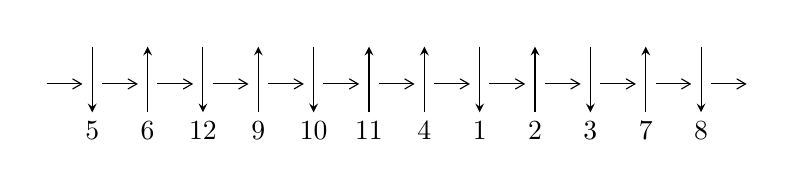
\begin{tikzpicture}[x=20pt, y=17pt]
	% nodes
	\node (C0) at (0, 0) {};
	\node (C1) at (1, 0) {};
	\node (C1U) at (1, +1) {};
	\node (C1D) at (1, -1) {5};

	\node (C2) at (2, 0) {};
	\node (C2U) at (2, +1) {};
	\node (C2D) at (2, -1) {6};

	\node (C3) at (3, 0) {};
	\node (C3U) at (3, +1) {};
	\node (C3D) at (3, -1) {12};

	\node (C4) at (4, 0) {};
	\node (C4U) at (4, +1) {};
	\node (C4D) at (4, -1) {9};

	\node (C5) at (5, 0) {};
	\node (C5U) at (5, +1) {};
	\node (C5D) at (5, -1) {10};

	\node (C6) at (6, 0) {};
	\node (C6U) at (6, +1) {};
	\node (C6D) at (6, -1) {11};

	\node (C7) at (7, 0) {};
	\node (C7U) at (7, +1) {};
	\node (C7D) at (7, -1) {4};

	\node (C8) at (8, 0) {};
	\node (C8U) at (8, +1) {};
	\node (C8D) at (8, -1) {1};

	\node (C9) at (9, 0) {};
	\node (C9U) at (9, +1) {};
	\node (C9D) at (9, -1) {2};

	\node (C10) at (10, 0) {};
	\node (C10U) at (10, +1) {};
	\node (C10D) at (10, -1) {3};

	\node (C11) at (11, 0) {};
	\node (C11U) at (11, +1) {};
	\node (C11D) at (11, -1) {7};

	\node (C12) at (12, 0) {};
	\node (C12U) at (12, +1) {};
	\node (C12D) at (12, -1) {8};
	\node (C13) at (13, 0) {};

	% arrows
	\draw[->,>={angle 60}]
	(C0) edge (C1) (C1) edge (C2) (C2) edge (C3) (C3) edge (C4) (C4) edge (C5) (C5) edge (C6) (C6) edge (C7) (C7) edge (C8) (C8) edge (C9) (C9) edge (C10) (C10) edge (C11) (C11) edge (C12) (C12) edge (C13) ;	\draw[->,>=stealth]
	(C1U) edge (C1D) (C2D) edge (C2U) (C3U) edge (C3D) (C4D) edge (C4U) (C5U) edge (C5D) (C6D) edge (C6U) (C7D) edge (C7U) (C8U) edge (C8D) (C9D) edge (C9U) (C10U) edge (C10D) (C11D) edge (C11U) (C12U) edge (C12D) ;
	\end{tikzpicture} \\
\hhline{~~} \\& 
\textbf{Solving Sequence} \\ \cline{2-2} 
 &
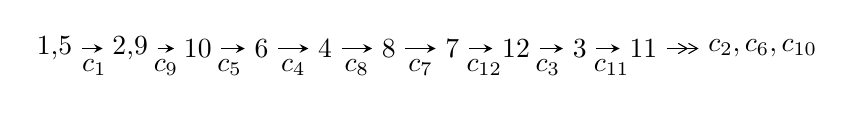
\begin{tikzpicture}[x=23pt, y=7pt]
	% node
	\node (A0) at (-1/8, 0) {1,5};
	\node (A1) at (17/16, 0) {2,9};
	\node (A2) at (17/8, 0) {10};
	\node (A3) at (25/8, 0) {6};
	\node (A4) at (33/8, 0) {4};
	\node (A5) at (41/8, 0) {8};
	\node (A6) at (49/8, 0) {7};
	\node (A7) at (57/8, 0) {12};
	\node (A8) at (65/8, 0) {3};
	\node (A9) at (73/8, 0) {11};
	\node (C1) at (1/2, -1) {$c_{1}$};
	\node (C2) at (13/8, -1) {$c_{9}$};
	\node (C3) at (21/8, -1) {$c_{5}$};
	\node (C4) at (29/8, -1) {$c_{4}$};
	\node (C5) at (37/8, -1) {$c_{8}$};
	\node (C6) at (45/8, -1) {$c_{7}$};
	\node (C7) at (53/8, -1) {$c_{12}$};
	\node (C8) at (61/8, -1) {$c_{3}$};
	\node (C9) at (69/8, -1) {$c_{11}$};
	\node (A10) at (11, 0) {$c_{2},c_{6},c_{10}$};

	% edge
	\draw[->,>=stealth]	
	(A0) edge (A1) (A1) edge (A2) (A2) edge (A3) (A3) edge (A4) (A4) edge (A5) (A5) edge (A6) (A6) edge (A7) (A7) edge (A8) (A8) edge (A9) ;
	\draw[->>,>={angle 60}]	
	(A9) edge (A10);
\end{tikzpicture} \\ 

\end{tabular} \\

\footnotetext{
The image of knot diagram is generated by the software ``\textbf{Draw programme}" developed by Andrew Bartholomew(\url{http://www.layer8.co.uk/maths/draw/index.htm\#Running-draw}), where we modified some parts for our purpose(\url{https://github.com/CATsTAILs/LinksPainter}).
}\phantom \\ \newline 
\centering \textbf{Ideals for irreducible components\footnotemark of $X_{\text{par}}$} 
 
\begin{align*}
I^u_{1}&=\langle 
1.05880\times10^{1211} u^{151}+2.26006\times10^{1211} u^{150}+\cdots+1.94891\times10^{1209} b-1.10493\times10^{1216},\\
\phantom{I^u_{1}}&\phantom{= \langle  }1.10741\times10^{1217} u^{151}+1.41825\times10^{1217} u^{150}+\cdots+7.44939\times10^{1212} a-5.29595\times10^{1221},\\
\phantom{I^u_{1}}&\phantom{= \langle  }3 u^{152}+6 u^{151}+\cdots-1329546 u-103203\rangle \\
I^u_{2}&=\langle 
3.30965\times10^{20} u^{23}+5.28416\times10^{20} u^{22}+\cdots+1.04360\times10^{20} b-5.11134\times10^{20},\\
\phantom{I^u_{2}}&\phantom{= \langle  }-1.66263\times10^{21} u^{23}-5.94003\times10^{21} u^{22}+\cdots+1.04360\times10^{20} a-2.53190\times10^{21},\\
\phantom{I^u_{2}}&\phantom{= \langle  }3 u^{24}+9 u^{23}+\cdots+2 u-1\rangle \\
\\
\end{align*}
\raggedright * 2 irreducible components of $\dim_{\mathbb{C}}=0$, with total 176 representations.\\
\footnotetext{All coefficients of polynomials are rational numbers. But the coefficients are sometimes approximated in decimal forms when there is not enough margin.}
\newpage
\renewcommand{\arraystretch}{1}
\centering \section*{I. $I^u_{1}= \langle 1.06\times10^{1211} u^{151}+2.26\times10^{1211} u^{150}+\cdots+1.95\times10^{1209} b-1.10\times10^{1216},\;1.11\times10^{1217} u^{151}+1.42\times10^{1217} u^{150}+\cdots+7.45\times10^{1212} a-5.30\times10^{1221},\;3 u^{152}+6 u^{151}+\cdots-1329546 u-103203 \rangle$}
\flushleft \textbf{(i) Arc colorings}\\
\begin{tabular}{m{7pt} m{180pt} m{7pt} m{180pt} }
\flushright $a_{1}=$&$\begin{pmatrix}1\\0\end{pmatrix}$ \\
\flushright $a_{5}=$&$\begin{pmatrix}0\\u\end{pmatrix}$ \\
\flushright $a_{2}=$&$\begin{pmatrix}1\\u^2\end{pmatrix}$ \\
\flushright $a_{9}=$&$\begin{pmatrix}-14865.8 u^{151}-19038.5 u^{150}+\cdots+8.17045\times10^{9} u+7.10924\times10^{8}\\-54.3277 u^{151}-115.965 u^{150}+\cdots+6.09045\times10^{7} u+5.66945\times10^{6}\end{pmatrix}$ \\
\flushright $a_{10}=$&$\begin{pmatrix}-7228.80 u^{151}-9303.61 u^{150}+\cdots+4.00373\times10^{9} u+3.48737\times10^{8}\\3962.88 u^{151}+5005.33 u^{150}+\cdots-2.13124\times10^{9} u-1.84884\times10^{8}\end{pmatrix}$ \\
\flushright $a_{6}=$&$\begin{pmatrix}-20077.4 u^{151}-25717.6 u^{150}+\cdots+1.10380\times10^{10} u+9.60477\times10^{8}\\-4996.99 u^{151}-6399.33 u^{150}+\cdots+2.74640\times10^{9} u+2.38970\times10^{8}\end{pmatrix}$ \\
\flushright $a_{4}=$&$\begin{pmatrix}-23946.1 u^{151}-30673.4 u^{150}+\cdots+1.31647\times10^{10} u+1.14552\times10^{9}\\-13896.0 u^{151}-17802.5 u^{150}+\cdots+7.64182\times10^{9} u+6.64983\times10^{8}\end{pmatrix}$ \\
\flushright $a_{8}=$&$\begin{pmatrix}-14920.1 u^{151}-19154.4 u^{150}+\cdots+8.23135\times10^{9} u+7.16593\times10^{8}\\-54.3277 u^{151}-115.965 u^{150}+\cdots+6.09045\times10^{7} u+5.66945\times10^{6}\end{pmatrix}$ \\
\flushright $a_{7}=$&$\begin{pmatrix}18958.2 u^{151}+24196.5 u^{150}+\cdots-1.03636\times10^{10} u-9.01066\times10^{8}\\8191.77 u^{151}+10493.9 u^{150}+\cdots-4.50345\times10^{9} u-3.91854\times10^{8}\end{pmatrix}$ \\
\flushright $a_{12}=$&$\begin{pmatrix}20806.2 u^{151}+26652.5 u^{150}+\cdots-1.14400\times10^{10} u-9.95476\times10^{8}\\1475.88 u^{151}+1887.91 u^{150}+\cdots-8.09724\times10^{8} u-7.04389\times10^{7}\end{pmatrix}$ \\
\flushright $a_{3}=$&$\begin{pmatrix}9044.11 u^{151}+11595.5 u^{150}+\cdots-4.98013\times10^{9} u-4.33451\times10^{8}\\-5100.12 u^{151}-6533.52 u^{150}+\cdots+2.80406\times10^{9} u+2.43992\times10^{8}\end{pmatrix}$ \\
\flushright $a_{11}=$&$\begin{pmatrix}17725.7 u^{151}+22622.6 u^{150}+\cdots-9.68954\times10^{9} u-8.42479\times10^{8}\\6973.18 u^{151}+8921.17 u^{150}+\cdots-3.82539\times10^{9} u-3.32753\times10^{8}\end{pmatrix}$\\&\end{tabular}
\flushleft \textbf{(ii) Obstruction class $= -1$}\\~\\
\flushleft \textbf{(iii) Cusp Shapes $= -43987.3 u^{151}-56280.9 u^{150}+\cdots+2.41418\times10^{10} u+2.10022\times10^{9}$}\\~\\
\newpage\renewcommand{\arraystretch}{1}
\flushleft \textbf{(iv) u-Polynomials at the component}\newline \\
\begin{tabular}{m{50pt}|m{274pt}}
Crossings & \hspace{64pt}u-Polynomials at each crossing \\
\hline $$\begin{aligned}c_{1}\end{aligned}$$&$\begin{aligned}
&3(3 u^{152}-6 u^{151}+\cdots+1329546 u-103203)
\end{aligned}$\\
\hline $$\begin{aligned}c_{2}\end{aligned}$$&$\begin{aligned}
&3(3 u^{152}+6 u^{151}+\cdots-1329546 u-103203)
\end{aligned}$\\
\hline $$\begin{aligned}c_{3}\end{aligned}$$&$\begin{aligned}
&u^{152}+2 u^{151}+\cdots-654 u+423
\end{aligned}$\\
\hline $$\begin{aligned}c_{4}\end{aligned}$$&$\begin{aligned}
&u^{152}+3 u^{151}+\cdots+13 u+1
\end{aligned}$\\
\hline $$\begin{aligned}c_{5}\end{aligned}$$&$\begin{aligned}
&u^{152}-9 u^{151}+\cdots+47757 u+7809
\end{aligned}$\\
\hline $$\begin{aligned}c_{6},c_{11}\end{aligned}$$&$\begin{aligned}
&3(3 u^{152}-167 u^{150}+\cdots-6 u+1)
\end{aligned}$\\
\hline $$\begin{aligned}c_{7}\end{aligned}$$&$\begin{aligned}
&u^{152}-2 u^{151}+\cdots+654 u+423
\end{aligned}$\\
\hline $$\begin{aligned}c_{8},c_{12}\end{aligned}$$&$\begin{aligned}
&3(3 u^{152}-167 u^{150}+\cdots+6 u+1)
\end{aligned}$\\
\hline $$\begin{aligned}c_{9}\end{aligned}$$&$\begin{aligned}
&u^{152}+9 u^{151}+\cdots-47757 u+7809
\end{aligned}$\\
\hline $$\begin{aligned}c_{10}\end{aligned}$$&$\begin{aligned}
&u^{152}-3 u^{151}+\cdots-13 u+1
\end{aligned}$\\
\hline
\end{tabular}\\~\\
\newpage\renewcommand{\arraystretch}{1}
\flushleft \textbf{(v) Riley Polynomials at the component}\newline \\
\begin{tabular}{m{50pt}|m{274pt}}
Crossings & \hspace{64pt}Riley Polynomials at each crossing \\
\hline $$\begin{aligned}c_{1},c_{2}\end{aligned}$$&$\begin{aligned}
&9(9 y^{152}-336 y^{151}+\cdots-7.13600\times10^{11} y+1.06509\times10^{10})
\end{aligned}$\\
\hline $$\begin{aligned}c_{3},c_{7}\end{aligned}$$&$\begin{aligned}
&y^{152}-42 y^{151}+\cdots+3035808 y+178929
\end{aligned}$\\
\hline $$\begin{aligned}c_{4},c_{10}\end{aligned}$$&$\begin{aligned}
&y^{152}-51 y^{151}+\cdots-1445 y+1
\end{aligned}$\\
\hline $$\begin{aligned}c_{5},c_{9}\end{aligned}$$&$\begin{aligned}
&y^{152}-57 y^{151}+\cdots-11081005509 y+60980481
\end{aligned}$\\
\hline $$\begin{aligned}c_{6},c_{8},c_{11}\\c_{12}\end{aligned}$$&$\begin{aligned}
&9(9 y^{152}-1002 y^{151}+\cdots-342 y+1)
\end{aligned}$\\
\hline
\end{tabular}\\~\\
\newpage\flushleft \textbf{(vi) Complex Volumes and Cusp Shapes}
$$\begin{array}{c|c|c}  
\text{Solutions to }I^u_{1}& \I (\text{vol} + \sqrt{-1}CS) & \text{Cusp shape}\\
 \hline 
\begin{aligned}
u &= -0.636691 + 0.751895 I \\
a &= \phantom{-}0.25274 - 1.64629 I \\
b &= -1.199820 + 0.107197 I\end{aligned}
 & -1.45660 + 1.48786 I & \phantom{-0.000000 } 0 \\ \hline\begin{aligned}
u &= -0.636691 - 0.751895 I \\
a &= \phantom{-}0.25274 + 1.64629 I \\
b &= -1.199820 - 0.107197 I\end{aligned}
 & -1.45660 - 1.48786 I & \phantom{-0.000000 } 0 \\ \hline\begin{aligned}
u &= -0.731220 + 0.713701 I \\
a &= -0.664353 - 0.881719 I \\
b &= \phantom{-}0.058799 + 0.702942 I\end{aligned}
 & \phantom{-}7.30912 - 0.08952 I & \phantom{-0.000000 } 0 \\ \hline\begin{aligned}
u &= -0.731220 - 0.713701 I \\
a &= -0.664353 + 0.881719 I \\
b &= \phantom{-}0.058799 - 0.702942 I\end{aligned}
 & \phantom{-}7.30912 + 0.08952 I & \phantom{-0.000000 } 0 \\ \hline\begin{aligned}
u &= -0.789031 + 0.535245 I \\
a &= -1.18743 - 0.96116 I \\
b &= -0.618641 + 0.493754 I\end{aligned}
 & \phantom{-}5.14963 - 0.61657 I & \phantom{-0.000000 } 0 \\ \hline\begin{aligned}
u &= -0.789031 - 0.535245 I \\
a &= -1.18743 + 0.96116 I \\
b &= -0.618641 - 0.493754 I\end{aligned}
 & \phantom{-}5.14963 + 0.61657 I & \phantom{-0.000000 } 0 \\ \hline\begin{aligned}
u &= \phantom{-}0.084639 + 0.948996 I \\
a &= \phantom{-}0.397571 + 0.845487 I \\
b &= \phantom{-}0.161590 - 0.798278 I\end{aligned}
 & \phantom{-}1.47653 - 1.54111 I & \phantom{-0.000000 } 0 \\ \hline\begin{aligned}
u &= \phantom{-}0.084639 - 0.948996 I \\
a &= \phantom{-}0.397571 - 0.845487 I \\
b &= \phantom{-}0.161590 + 0.798278 I\end{aligned}
 & \phantom{-}1.47653 + 1.54111 I & \phantom{-0.000000 } 0 \\ \hline\begin{aligned}
u &= \phantom{-}0.805693 + 0.672336 I \\
a &= -0.458714 - 0.915392 I \\
b &= \phantom{-}1.076740 + 0.628879 I\end{aligned}
 & \phantom{-}0.04971 - 3.50428 I & \phantom{-0.000000 } 0 \\ \hline\begin{aligned}
u &= \phantom{-}0.805693 - 0.672336 I \\
a &= -0.458714 + 0.915392 I \\
b &= \phantom{-}1.076740 - 0.628879 I\end{aligned}
 & \phantom{-}0.04971 + 3.50428 I & \phantom{-0.000000 } 0\\
 \hline 
 \end{array}$$\newpage$$\begin{array}{c|c|c}  
\text{Solutions to }I^u_{1}& \I (\text{vol} + \sqrt{-1}CS) & \text{Cusp shape}\\
 \hline 
\begin{aligned}
u &= \phantom{-}0.945821 + 0.056351 I \\
a &= -1.15996 + 1.37999 I \\
b &= -1.171130 + 0.127953 I\end{aligned}
 & -3.38143 + 3.80820 I & \phantom{-0.000000 } 0 \\ \hline\begin{aligned}
u &= \phantom{-}0.945821 - 0.056351 I \\
a &= -1.15996 - 1.37999 I \\
b &= -1.171130 - 0.127953 I\end{aligned}
 & -3.38143 - 3.80820 I & \phantom{-0.000000 } 0 \\ \hline\begin{aligned}
u &= -0.852982 + 0.617291 I \\
a &= \phantom{-}0.57651 + 1.53519 I \\
b &= \phantom{-}1.163850 - 0.350561 I\end{aligned}
 & \phantom{-}4.05943 + 3.77468 I & \phantom{-0.000000 } 0 \\ \hline\begin{aligned}
u &= -0.852982 - 0.617291 I \\
a &= \phantom{-}0.57651 - 1.53519 I \\
b &= \phantom{-}1.163850 + 0.350561 I\end{aligned}
 & \phantom{-}4.05943 - 3.77468 I & \phantom{-0.000000 } 0 \\ \hline\begin{aligned}
u &= \phantom{-}1.009200 + 0.310926 I \\
a &= \phantom{-}0.045338 + 1.054200 I \\
b &= -1.332530 - 0.121288 I\end{aligned}
 & -4.05943 - 3.77468 I & \phantom{-0.000000 } 0 \\ \hline\begin{aligned}
u &= \phantom{-}1.009200 - 0.310926 I \\
a &= \phantom{-}0.045338 - 1.054200 I \\
b &= -1.332530 + 0.121288 I\end{aligned}
 & -4.05943 + 3.77468 I & \phantom{-0.000000 } 0 \\ \hline\begin{aligned}
u &= -0.913241 + 0.236199 I \\
a &= -0.29195 - 1.63189 I \\
b &= -1.39666 + 0.47368 I\end{aligned}
 & -2.60387 + 11.50010 I & \phantom{-0.000000 } 0 \\ \hline\begin{aligned}
u &= -0.913241 - 0.236199 I \\
a &= -0.29195 + 1.63189 I \\
b &= -1.39666 - 0.47368 I\end{aligned}
 & -2.60387 - 11.50010 I & \phantom{-0.000000 } 0 \\ \hline\begin{aligned}
u &= \phantom{-}0.928790 + 0.154523 I \\
a &= \phantom{-}0.43162 - 3.30454 I \\
b &= \phantom{-}0.993981 + 0.166281 I\end{aligned}
 & \phantom{-}1.58030 - 0.46294 I & \phantom{-0.000000 } 0 \\ \hline\begin{aligned}
u &= \phantom{-}0.928790 - 0.154523 I \\
a &= \phantom{-}0.43162 + 3.30454 I \\
b &= \phantom{-}0.993981 - 0.166281 I\end{aligned}
 & \phantom{-}1.58030 + 0.46294 I & \phantom{-0.000000 } 0\\
 \hline 
 \end{array}$$\newpage$$\begin{array}{c|c|c}  
\text{Solutions to }I^u_{1}& \I (\text{vol} + \sqrt{-1}CS) & \text{Cusp shape}\\
 \hline 
\begin{aligned}
u &= \phantom{-}1.066520 + 0.152455 I \\
a &= \phantom{-}0.555153 - 0.959621 I \\
b &= \phantom{-}1.294750 - 0.030630 I\end{aligned}
 & -7.30912 + 0.08952 I & \phantom{-0.000000 } 0 \\ \hline\begin{aligned}
u &= \phantom{-}1.066520 - 0.152455 I \\
a &= \phantom{-}0.555153 + 0.959621 I \\
b &= \phantom{-}1.294750 + 0.030630 I\end{aligned}
 & -7.30912 - 0.08952 I & \phantom{-0.000000 } 0 \\ \hline\begin{aligned}
u &= \phantom{-}0.495469 + 0.774065 I \\
a &= \phantom{-}0.010206 - 0.369341 I \\
b &= -0.96174 + 1.12426 I\end{aligned}
 & \phantom{-}3.39442 - 6.97676 I & \phantom{-0.000000 } 0 \\ \hline\begin{aligned}
u &= \phantom{-}0.495469 - 0.774065 I \\
a &= \phantom{-}0.010206 + 0.369341 I \\
b &= -0.96174 - 1.12426 I\end{aligned}
 & \phantom{-}3.39442 + 6.97676 I & \phantom{-0.000000 } 0 \\ \hline\begin{aligned}
u &= \phantom{-}0.516183 + 0.952324 I \\
a &= \phantom{-}0.096371 - 1.136120 I \\
b &= \phantom{-}0.171266 + 0.931919 I\end{aligned}
 & \phantom{-}7.58787 - 6.67654 I & \phantom{-0.000000 } 0 \\ \hline\begin{aligned}
u &= \phantom{-}0.516183 - 0.952324 I \\
a &= \phantom{-}0.096371 + 1.136120 I \\
b &= \phantom{-}0.171266 - 0.931919 I\end{aligned}
 & \phantom{-}7.58787 + 6.67654 I & \phantom{-0.000000 } 0 \\ \hline\begin{aligned}
u &= \phantom{-}0.759634 + 0.512391 I \\
a &= -0.70862 - 2.12763 I \\
b &= \phantom{-}1.164990 - 0.017764 I\end{aligned}
 & \phantom{-0.000000 } -1.02020 I & \phantom{-0.000000 } 0 \\ \hline\begin{aligned}
u &= \phantom{-}0.759634 - 0.512391 I \\
a &= -0.70862 + 2.12763 I \\
b &= \phantom{-}1.164990 + 0.017764 I\end{aligned}
 & \phantom{-0.000000 -}1.02020 I & \phantom{-0.000000 } 0 \\ \hline\begin{aligned}
u &= \phantom{-}1.08633\phantom{ +0.000000I} \\
a &= \phantom{-}6.50562\phantom{ +0.000000I} \\
b &= \phantom{-}1.05342\phantom{ +0.000000I}\end{aligned}
 & \phantom{-}1.48784\phantom{ +0.000000I} & \phantom{-0.000000 } 0 \\ \hline\begin{aligned}
u &= -0.880859 + 0.241700 I \\
a &= \phantom{-}0.39390 + 1.42044 I \\
b &= \phantom{-}1.45856 - 0.42854 I\end{aligned}
 & -7.58787 + 6.67654 I & \phantom{-0.000000 } 0\\
 \hline 
 \end{array}$$\newpage$$\begin{array}{c|c|c}  
\text{Solutions to }I^u_{1}& \I (\text{vol} + \sqrt{-1}CS) & \text{Cusp shape}\\
 \hline 
\begin{aligned}
u &= -0.880859 - 0.241700 I \\
a &= \phantom{-}0.39390 - 1.42044 I \\
b &= \phantom{-}1.45856 + 0.42854 I\end{aligned}
 & -7.58787 - 6.67654 I & \phantom{-0.000000 } 0 \\ \hline\begin{aligned}
u &= -0.807025 + 0.728809 I \\
a &= -0.164578 - 0.800281 I \\
b &= -0.106801 + 1.283040 I\end{aligned}
 & \phantom{-}1.39846 + 5.82902 I & \phantom{-0.000000 } 0 \\ \hline\begin{aligned}
u &= -0.807025 - 0.728809 I \\
a &= -0.164578 + 0.800281 I \\
b &= -0.106801 - 1.283040 I\end{aligned}
 & \phantom{-}1.39846 - 5.82902 I & \phantom{-0.000000 } 0 \\ \hline\begin{aligned}
u &= \phantom{-}0.498989 + 0.749781 I \\
a &= \phantom{-}0.405769 + 0.535961 I \\
b &= \phantom{-}0.159058 - 0.589326 I\end{aligned}
 & \phantom{-0.000000 } -1.79018 I & \phantom{-0.000000 } 0 \\ \hline\begin{aligned}
u &= \phantom{-}0.498989 - 0.749781 I \\
a &= \phantom{-}0.405769 - 0.535961 I \\
b &= \phantom{-}0.159058 + 0.589326 I\end{aligned}
 & \phantom{-0.000000 -}1.79018 I & \phantom{-0.000000 } 0 \\ \hline\begin{aligned}
u &= -0.890726 + 0.645966 I \\
a &= \phantom{-}0.425517 - 1.074820 I \\
b &= -0.1035150 + 0.0576443 I\end{aligned}
 & \phantom{-}1.72248 + 9.63955 I & \phantom{-0.000000 } 0 \\ \hline\begin{aligned}
u &= -0.890726 - 0.645966 I \\
a &= \phantom{-}0.425517 + 1.074820 I \\
b &= -0.1035150 - 0.0576443 I\end{aligned}
 & \phantom{-}1.72248 - 9.63955 I & \phantom{-0.000000 } 0 \\ \hline\begin{aligned}
u &= \phantom{-}1.10899\phantom{ +0.000000I} \\
a &= \phantom{-}0.611931\phantom{ +0.000000I} \\
b &= -0.365730\phantom{ +0.000000I}\end{aligned}
 & -2.37631\phantom{ +0.000000I} & \phantom{-0.000000 } 0 \\ \hline\begin{aligned}
u &= -0.891587 + 0.661946 I \\
a &= \phantom{-}0.279865 + 0.850269 I \\
b &= -0.390414 - 1.050390 I\end{aligned}
 & \phantom{-}4.91380 + 5.50279 I & \phantom{-0.000000 } 0 \\ \hline\begin{aligned}
u &= -0.891587 - 0.661946 I \\
a &= \phantom{-}0.279865 - 0.850269 I \\
b &= -0.390414 + 1.050390 I\end{aligned}
 & \phantom{-}4.91380 - 5.50279 I & \phantom{-0.000000 } 0\\
 \hline 
 \end{array}$$\newpage$$\begin{array}{c|c|c}  
\text{Solutions to }I^u_{1}& \I (\text{vol} + \sqrt{-1}CS) & \text{Cusp shape}\\
 \hline 
\begin{aligned}
u &= -0.721286 + 0.512414 I \\
a &= -0.226659 - 0.405159 I \\
b &= \phantom{-}1.039650 + 0.476428 I\end{aligned}
 & \phantom{-}4.19522 + 0.69390 I & \phantom{-0.000000 } 0 \\ \hline\begin{aligned}
u &= -0.721286 - 0.512414 I \\
a &= -0.226659 + 0.405159 I \\
b &= \phantom{-}1.039650 - 0.476428 I\end{aligned}
 & \phantom{-}4.19522 - 0.69390 I & \phantom{-0.000000 } 0 \\ \hline\begin{aligned}
u &= \phantom{-}0.933420 + 0.646785 I \\
a &= \phantom{-}0.403691 + 0.631654 I \\
b &= -0.253039 - 0.049643 I\end{aligned}
 & -0.61911 - 2.78150 I & \phantom{-0.000000 } 0 \\ \hline\begin{aligned}
u &= \phantom{-}0.933420 - 0.646785 I \\
a &= \phantom{-}0.403691 - 0.631654 I \\
b &= -0.253039 + 0.049643 I\end{aligned}
 & -0.61911 + 2.78150 I & \phantom{-0.000000 } 0 \\ \hline\begin{aligned}
u &= -0.899372 + 0.694857 I \\
a &= -0.230688 - 0.889354 I \\
b &= \phantom{-}0.059423 + 0.929752 I\end{aligned}
 & \phantom{-}2.15753 + 4.93327 I & \phantom{-0.000000 } 0 \\ \hline\begin{aligned}
u &= -0.899372 - 0.694857 I \\
a &= -0.230688 + 0.889354 I \\
b &= \phantom{-}0.059423 - 0.929752 I\end{aligned}
 & \phantom{-}2.15753 - 4.93327 I & \phantom{-0.000000 } 0 \\ \hline\begin{aligned}
u &= \phantom{-}0.854268 + 0.758556 I \\
a &= \phantom{-}0.285556 + 0.876813 I \\
b &= -0.695108 - 0.641861 I\end{aligned}
 & -0.22990 - 2.73957 I & \phantom{-0.000000 } 0 \\ \hline\begin{aligned}
u &= \phantom{-}0.854268 - 0.758556 I \\
a &= \phantom{-}0.285556 - 0.876813 I \\
b &= -0.695108 + 0.641861 I\end{aligned}
 & -0.22990 + 2.73957 I & \phantom{-0.000000 } 0 \\ \hline\begin{aligned}
u &= -0.816605 + 0.243167 I \\
a &= -0.634800 - 1.109670 I \\
b &= -1.51259 + 0.33584 I\end{aligned}
 & -4.64789 + 1.50476 I & \phantom{-0.000000 } 0 \\ \hline\begin{aligned}
u &= -0.816605 - 0.243167 I \\
a &= -0.634800 + 1.109670 I \\
b &= -1.51259 - 0.33584 I\end{aligned}
 & -4.64789 - 1.50476 I & \phantom{-0.000000 } 0\\
 \hline 
 \end{array}$$\newpage$$\begin{array}{c|c|c}  
\text{Solutions to }I^u_{1}& \I (\text{vol} + \sqrt{-1}CS) & \text{Cusp shape}\\
 \hline 
\begin{aligned}
u &= -0.843788\phantom{ +0.000000I} \\
a &= \phantom{-}0.0325475\phantom{ +0.000000I} \\
b &= \phantom{-}1.84418\phantom{ +0.000000I}\end{aligned}
 & -3.40001\phantom{ +0.000000I} & \phantom{-0.000000 } 0 \\ \hline\begin{aligned}
u &= -0.897255 + 0.740465 I \\
a &= -0.393272 + 0.603493 I \\
b &= -0.241623 + 0.009695 I\end{aligned}
 & -2.15753 + 4.93327 I & \phantom{-0.000000 } 0 \\ \hline\begin{aligned}
u &= -0.897255 - 0.740465 I \\
a &= -0.393272 - 0.603493 I \\
b &= -0.241623 - 0.009695 I\end{aligned}
 & -2.15753 - 4.93327 I & \phantom{-0.000000 } 0 \\ \hline\begin{aligned}
u &= \phantom{-}0.800657 + 0.211797 I \\
a &= -0.01681 + 2.46647 I \\
b &= -1.124590 - 0.178093 I\end{aligned}
 & -3.05517 - 0.85011 I & \phantom{-0.000000 } 0 \\ \hline\begin{aligned}
u &= \phantom{-}0.800657 - 0.211797 I \\
a &= -0.01681 - 2.46647 I \\
b &= -1.124590 + 0.178093 I\end{aligned}
 & -3.05517 + 0.85011 I & \phantom{-0.000000 } 0 \\ \hline\begin{aligned}
u &= \phantom{-}1.160810 + 0.178463 I \\
a &= \phantom{-}0.247574 - 0.306571 I \\
b &= -0.282293 + 0.050532 I\end{aligned}
 & -2.38361 - 0.03883 I & \phantom{-0.000000 } 0 \\ \hline\begin{aligned}
u &= \phantom{-}1.160810 - 0.178463 I \\
a &= \phantom{-}0.247574 + 0.306571 I \\
b &= -0.282293 - 0.050532 I\end{aligned}
 & -2.38361 + 0.03883 I & \phantom{-0.000000 } 0 \\ \hline\begin{aligned}
u &= -0.485978 + 1.071620 I \\
a &= \phantom{-}0.448650 + 0.443440 I \\
b &= -0.730761 - 0.451693 I\end{aligned}
 & \phantom{-}4.84181 - 4.51668 I & \phantom{-0.000000 } 0 \\ \hline\begin{aligned}
u &= -0.485978 - 1.071620 I \\
a &= \phantom{-}0.448650 - 0.443440 I \\
b &= -0.730761 + 0.451693 I\end{aligned}
 & \phantom{-}4.84181 + 4.51668 I & \phantom{-0.000000 } 0 \\ \hline\begin{aligned}
u &= \phantom{-}0.819600 + 0.063753 I \\
a &= -0.249531 + 1.353600 I \\
b &= \phantom{-}0.438924 - 0.619311 I\end{aligned}
 & \phantom{-}1.45660 + 1.48786 I & \phantom{-0.000000 } 0\\
 \hline 
 \end{array}$$\newpage$$\begin{array}{c|c|c}  
\text{Solutions to }I^u_{1}& \I (\text{vol} + \sqrt{-1}CS) & \text{Cusp shape}\\
 \hline 
\begin{aligned}
u &= \phantom{-}0.819600 - 0.063753 I \\
a &= -0.249531 - 1.353600 I \\
b &= \phantom{-}0.438924 + 0.619311 I\end{aligned}
 & \phantom{-}1.45660 - 1.48786 I & \phantom{-0.000000 } 0 \\ \hline\begin{aligned}
u &= -0.925365 + 0.737997 I \\
a &= \phantom{-}0.344697 + 1.021700 I \\
b &= \phantom{-}0.188307 - 0.905744 I\end{aligned}
 & \phantom{-}6.86103 + 5.62133 I & \phantom{-0.000000 } 0 \\ \hline\begin{aligned}
u &= -0.925365 - 0.737997 I \\
a &= \phantom{-}0.344697 - 1.021700 I \\
b &= \phantom{-}0.188307 + 0.905744 I\end{aligned}
 & \phantom{-}6.86103 - 5.62133 I & \phantom{-0.000000 } 0 \\ \hline\begin{aligned}
u &= -0.809191\phantom{ +0.000000I} \\
a &= -1.80913\phantom{ +0.000000I} \\
b &= \phantom{-}0.118236\phantom{ +0.000000I}\end{aligned}
 & \phantom{-}8.08455\phantom{ +0.000000I} & \phantom{-0.000000 } 0 \\ \hline\begin{aligned}
u &= -0.726709 + 0.354257 I \\
a &= \phantom{-}1.20067 + 0.75389 I \\
b &= \phantom{-}0.297738 - 0.279599 I\end{aligned}
 & \phantom{-}2.38361 - 0.03883 I & \phantom{-0.000000 } 0 \\ \hline\begin{aligned}
u &= -0.726709 - 0.354257 I \\
a &= \phantom{-}1.20067 - 0.75389 I \\
b &= \phantom{-}0.297738 + 0.279599 I\end{aligned}
 & \phantom{-}2.38361 + 0.03883 I & \phantom{-0.000000 } 0 \\ \hline\begin{aligned}
u &= -0.787310\phantom{ +0.000000I} \\
a &= -0.370932\phantom{ +0.000000I} \\
b &= -1.68866\phantom{ +0.000000I}\end{aligned}
 & -4.12835\phantom{ +0.000000I} & \phantom{-0.000000 } 0 \\ \hline\begin{aligned}
u &= -0.648727 + 1.033260 I \\
a &= \phantom{-}0.426711 + 0.104654 I \\
b &= -1.246010 - 0.324832 I\end{aligned}
 & \phantom{-}3.38143 - 3.80820 I & \phantom{-0.000000 } 0 \\ \hline\begin{aligned}
u &= -0.648727 - 1.033260 I \\
a &= \phantom{-}0.426711 - 0.104654 I \\
b &= -1.246010 + 0.324832 I\end{aligned}
 & \phantom{-}3.38143 + 3.80820 I & \phantom{-0.000000 } 0 \\ \hline\begin{aligned}
u &= -0.737557 + 0.032144 I \\
a &= -0.84339 - 2.51654 I \\
b &= -1.236740 - 0.108960 I\end{aligned}
 & -1.82737 - 10.33300 I & \phantom{-0.000000 } 0\\
 \hline 
 \end{array}$$\newpage$$\begin{array}{c|c|c}  
\text{Solutions to }I^u_{1}& \I (\text{vol} + \sqrt{-1}CS) & \text{Cusp shape}\\
 \hline 
\begin{aligned}
u &= -0.737557 - 0.032144 I \\
a &= -0.84339 + 2.51654 I \\
b &= -1.236740 + 0.108960 I\end{aligned}
 & -1.82737 + 10.33300 I & \phantom{-0.000000 } 0 \\ \hline\begin{aligned}
u &= -0.720495 + 0.002427 I \\
a &= \phantom{-}1.12155 + 2.01585 I \\
b &= \phantom{-}1.288740 + 0.078429 I\end{aligned}
 & -6.86103 - 5.62133 I & \phantom{-0.000000 } 0 \\ \hline\begin{aligned}
u &= -0.720495 - 0.002427 I \\
a &= \phantom{-}1.12155 - 2.01585 I \\
b &= \phantom{-}1.288740 - 0.078429 I\end{aligned}
 & -6.86103 + 5.62133 I & \phantom{-0.000000 } 0 \\ \hline\begin{aligned}
u &= -0.428344 + 1.214070 I \\
a &= -0.287209 - 0.158425 I \\
b &= \phantom{-}1.011590 + 0.209467 I\end{aligned}
 & \phantom{-}0.61911 - 2.78150 I & \phantom{-0.000000 } 0 \\ \hline\begin{aligned}
u &= -0.428344 - 1.214070 I \\
a &= -0.287209 + 0.158425 I \\
b &= \phantom{-}1.011590 - 0.209467 I\end{aligned}
 & \phantom{-}0.61911 + 2.78150 I & \phantom{-0.000000 } 0 \\ \hline\begin{aligned}
u &= -0.710358 + 0.032872 I \\
a &= -1.14133 + 1.08383 I \\
b &= -1.372780 + 0.004924 I\end{aligned}
 & -4.19522 + 0.69390 I & \phantom{-0.000000 } 0 \\ \hline\begin{aligned}
u &= -0.710358 - 0.032872 I \\
a &= -1.14133 - 1.08383 I \\
b &= -1.372780 - 0.004924 I\end{aligned}
 & -4.19522 - 0.69390 I & \phantom{-0.000000 } 0 \\ \hline\begin{aligned}
u &= \phantom{-}0.858181 + 0.965391 I \\
a &= \phantom{-}0.001584 + 1.267320 I \\
b &= -1.40518 - 0.41108 I\end{aligned}
 & \phantom{-}2.60387 - 11.50010 I & \phantom{-0.000000 } 0 \\ \hline\begin{aligned}
u &= \phantom{-}0.858181 - 0.965391 I \\
a &= \phantom{-}0.001584 - 1.267320 I \\
b &= -1.40518 + 0.41108 I\end{aligned}
 & \phantom{-}2.60387 + 11.50010 I & \phantom{-0.000000 } 0 \\ \hline\begin{aligned}
u &= -1.31401\phantom{ +0.000000I} \\
a &= -0.330378\phantom{ +0.000000I} \\
b &= \phantom{-}0.870071\phantom{ +0.000000I}\end{aligned}
 & \phantom{-}4.12835\phantom{ +0.000000I} & \phantom{-0.000000 } 0\\
 \hline 
 \end{array}$$\newpage$$\begin{array}{c|c|c}  
\text{Solutions to }I^u_{1}& \I (\text{vol} + \sqrt{-1}CS) & \text{Cusp shape}\\
 \hline 
\begin{aligned}
u &= -0.350825 + 0.587374 I \\
a &= \phantom{-}1.049160 + 0.590441 I \\
b &= \phantom{-}0.281515 - 0.543907 I\end{aligned}
 & \phantom{-}1.52906 - 1.26531 I & \phantom{-0.000000 } 0 \\ \hline\begin{aligned}
u &= -0.350825 - 0.587374 I \\
a &= \phantom{-}1.049160 - 0.590441 I \\
b &= \phantom{-}0.281515 + 0.543907 I\end{aligned}
 & \phantom{-}1.52906 + 1.26531 I & \phantom{-0.000000 } 0 \\ \hline\begin{aligned}
u &= \phantom{-}0.661940 + 0.064824 I \\
a &= -0.32617 - 1.44844 I \\
b &= -1.39529 + 0.73494 I\end{aligned}
 & -2.13670 + 3.65468 I & \phantom{-0.000000 } 0 \\ \hline\begin{aligned}
u &= \phantom{-}0.661940 - 0.064824 I \\
a &= -0.32617 + 1.44844 I \\
b &= -1.39529 - 0.73494 I\end{aligned}
 & -2.13670 - 3.65468 I & \phantom{-0.000000 } 0 \\ \hline\begin{aligned}
u &= \phantom{-}0.043716 + 0.662779 I \\
a &= -0.093280 + 1.139950 I \\
b &= \phantom{-}1.138900 - 0.538085 I\end{aligned}
 & \phantom{-}4.64789 - 1.50476 I & \phantom{-0.000000 } 0 \\ \hline\begin{aligned}
u &= \phantom{-}0.043716 - 0.662779 I \\
a &= -0.093280 - 1.139950 I \\
b &= \phantom{-}1.138900 + 0.538085 I\end{aligned}
 & \phantom{-}4.64789 + 1.50476 I & \phantom{-0.000000 } 0 \\ \hline\begin{aligned}
u &= \phantom{-}1.34295\phantom{ +0.000000I} \\
a &= \phantom{-}0.560443\phantom{ +0.000000I} \\
b &= \phantom{-}1.42045\phantom{ +0.000000I}\end{aligned}
 & -8.08455\phantom{ +0.000000I} & \phantom{-0.000000 } 0 \\ \hline\begin{aligned}
u &= -1.128690 + 0.768112 I \\
a &= -0.249179 - 1.375290 I \\
b &= -1.40484 + 0.40131 I\end{aligned}
 & \phantom{-}1.82737 + 10.33300 I & \phantom{-0.000000 } 0 \\ \hline\begin{aligned}
u &= -1.128690 - 0.768112 I \\
a &= -0.249179 + 1.375290 I \\
b &= -1.40484 - 0.40131 I\end{aligned}
 & \phantom{-}1.82737 - 10.33300 I & \phantom{-0.000000 } 0 \\ \hline\begin{aligned}
u &= -0.577775 + 0.209403 I \\
a &= \phantom{-}0.800729 - 0.650904 I \\
b &= \phantom{-}0.104817 + 1.030250 I\end{aligned}
 & \phantom{-}2.16133 - 6.12521 I & \phantom{-0.000000 } 0\\
 \hline 
 \end{array}$$\newpage$$\begin{array}{c|c|c}  
\text{Solutions to }I^u_{1}& \I (\text{vol} + \sqrt{-1}CS) & \text{Cusp shape}\\
 \hline 
\begin{aligned}
u &= -0.577775 - 0.209403 I \\
a &= \phantom{-}0.800729 + 0.650904 I \\
b &= \phantom{-}0.104817 - 1.030250 I\end{aligned}
 & \phantom{-}2.16133 + 6.12521 I & \phantom{-0.000000 } 0 \\ \hline\begin{aligned}
u &= -1.184700 + 0.730411 I \\
a &= -0.257040 - 1.243740 I \\
b &= -1.083630 + 0.502462 I\end{aligned}
 & \phantom{-}2.67378 + 10.96210 I & \phantom{-0.000000 } 0 \\ \hline\begin{aligned}
u &= -1.184700 - 0.730411 I \\
a &= -0.257040 + 1.243740 I \\
b &= -1.083630 - 0.502462 I\end{aligned}
 & \phantom{-}2.67378 - 10.96210 I & \phantom{-0.000000 } 0 \\ \hline\begin{aligned}
u &= \phantom{-}1.051740 + 0.918641 I \\
a &= -0.241001 + 0.803338 I \\
b &= -0.283863 - 1.172900 I\end{aligned}
 & \phantom{-}5.4746 - 14.2754 I & \phantom{-0.000000 } 0 \\ \hline\begin{aligned}
u &= \phantom{-}1.051740 - 0.918641 I \\
a &= -0.241001 - 0.803338 I \\
b &= -0.283863 + 1.172900 I\end{aligned}
 & \phantom{-}5.4746 + 14.2754 I & \phantom{-0.000000 } 0 \\ \hline\begin{aligned}
u &= \phantom{-}1.00309 + 1.01079 I \\
a &= \phantom{-}0.143887 - 0.716339 I \\
b &= \phantom{-}0.321664 + 1.158560 I\end{aligned}
 & \phantom{-0.000000 } -8.49285 I & \phantom{-0.000000 } 0 \\ \hline\begin{aligned}
u &= \phantom{-}1.00309 - 1.01079 I \\
a &= \phantom{-}0.143887 + 0.716339 I \\
b &= \phantom{-}0.321664 - 1.158560 I\end{aligned}
 & \phantom{-0.000000 -}8.49285 I & \phantom{-0.000000 } 0 \\ \hline\begin{aligned}
u &= -1.20876 + 0.76953 I \\
a &= \phantom{-}0.236739 + 1.208780 I \\
b &= \phantom{-}1.288130 - 0.403420 I\end{aligned}
 & -1.72248 + 9.63955 I & \phantom{-0.000000 } 0 \\ \hline\begin{aligned}
u &= -1.20876 - 0.76953 I \\
a &= \phantom{-}0.236739 - 1.208780 I \\
b &= \phantom{-}1.288130 + 0.403420 I\end{aligned}
 & -1.72248 - 9.63955 I & \phantom{-0.000000 } 0 \\ \hline\begin{aligned}
u &= \phantom{-}0.79111 + 1.20705 I \\
a &= \phantom{-}0.361988 - 0.605250 I \\
b &= \phantom{-}0.241067 + 1.026750 I\end{aligned}
 & \phantom{-}6.32408 + 6.86986 I & \phantom{-0.000000 } 0\\
 \hline 
 \end{array}$$\newpage$$\begin{array}{c|c|c}  
\text{Solutions to }I^u_{1}& \I (\text{vol} + \sqrt{-1}CS) & \text{Cusp shape}\\
 \hline 
\begin{aligned}
u &= \phantom{-}0.79111 - 1.20705 I \\
a &= \phantom{-}0.361988 + 0.605250 I \\
b &= \phantom{-}0.241067 - 1.026750 I\end{aligned}
 & \phantom{-}6.32408 - 6.86986 I & \phantom{-0.000000 } 0 \\ \hline\begin{aligned}
u &= \phantom{-}0.245134 + 0.497972 I \\
a &= \phantom{-}4.11437 + 3.18869 I \\
b &= -1.368890 - 0.032325 I\end{aligned}
 & -1.58030 + 0.46294 I & \phantom{-0.000000 } 0 \\ \hline\begin{aligned}
u &= \phantom{-}0.245134 - 0.497972 I \\
a &= \phantom{-}4.11437 - 3.18869 I \\
b &= -1.368890 + 0.032325 I\end{aligned}
 & -1.58030 - 0.46294 I & \phantom{-0.000000 } 0 \\ \hline\begin{aligned}
u &= \phantom{-}0.93457 + 1.12100 I \\
a &= -0.090695 - 0.901901 I \\
b &= \phantom{-}1.284930 + 0.421779 I\end{aligned}
 & -2.16133 - 6.12521 I & \phantom{-0.000000 } 0 \\ \hline\begin{aligned}
u &= \phantom{-}0.93457 - 1.12100 I \\
a &= -0.090695 + 0.901901 I \\
b &= \phantom{-}1.284930 - 0.421779 I\end{aligned}
 & -2.16133 + 6.12521 I & \phantom{-0.000000 } 0 \\ \hline\begin{aligned}
u &= \phantom{-}0.04389 + 1.47330 I \\
a &= -0.294729 - 0.207666 I \\
b &= \phantom{-}0.962214 + 0.418918 I\end{aligned}
 & \phantom{-0.000000 } -4.81270 I & \phantom{-0.000000 } 0 \\ \hline\begin{aligned}
u &= \phantom{-}0.04389 - 1.47330 I \\
a &= -0.294729 + 0.207666 I \\
b &= \phantom{-}0.962214 - 0.418918 I\end{aligned}
 & \phantom{-0.000000 -}4.81270 I & \phantom{-0.000000 } 0 \\ \hline\begin{aligned}
u &= \phantom{-}0.519830 + 0.015541 I \\
a &= \phantom{-}1.24237 + 1.09659 I \\
b &= \phantom{-}1.73677 - 0.38370 I\end{aligned}
 & -4.61027 + 0.46725 I & \phantom{-0.000000 } 0 \\ \hline\begin{aligned}
u &= \phantom{-}0.519830 - 0.015541 I \\
a &= \phantom{-}1.24237 - 1.09659 I \\
b &= \phantom{-}1.73677 + 0.38370 I\end{aligned}
 & -4.61027 - 0.46725 I & \phantom{-0.000000 } 0 \\ \hline\begin{aligned}
u &= -1.28521 + 0.79379 I \\
a &= \phantom{-}0.226798 + 0.997773 I \\
b &= \phantom{-}1.43430 - 0.56296 I\end{aligned}
 & -3.41653 + 12.20260 I & \phantom{-0.000000 } 0\\
 \hline 
 \end{array}$$\newpage$$\begin{array}{c|c|c}  
\text{Solutions to }I^u_{1}& \I (\text{vol} + \sqrt{-1}CS) & \text{Cusp shape}\\
 \hline 
\begin{aligned}
u &= -1.28521 - 0.79379 I \\
a &= \phantom{-}0.226798 - 0.997773 I \\
b &= \phantom{-}1.43430 + 0.56296 I\end{aligned}
 & -3.41653 - 12.20260 I & \phantom{-0.000000 } 0 \\ \hline\begin{aligned}
u &= \phantom{-}0.19157 + 1.50400 I \\
a &= -0.212998 + 0.313651 I \\
b &= \phantom{-}1.169330 - 0.495890 I\end{aligned}
 & \phantom{-}3.41653 + 12.20260 I & \phantom{-0.000000 } 0 \\ \hline\begin{aligned}
u &= \phantom{-}0.19157 - 1.50400 I \\
a &= -0.212998 - 0.313651 I \\
b &= \phantom{-}1.169330 + 0.495890 I\end{aligned}
 & \phantom{-}3.41653 - 12.20260 I & \phantom{-0.000000 } 0 \\ \hline\begin{aligned}
u &= -0.480973\phantom{ +0.000000I} \\
a &= \phantom{-}2.88668\phantom{ +0.000000I} \\
b &= \phantom{-}0.106217\phantom{ +0.000000I}\end{aligned}
 & \phantom{-}2.37631\phantom{ +0.000000I} & \phantom{-0.000000 } 0 \\ \hline\begin{aligned}
u &= \phantom{-}0.117245 + 0.451249 I \\
a &= \phantom{-}0.927082 - 0.011692 I \\
b &= -0.996224 - 0.461130 I\end{aligned}
 & -1.52906 - 1.26531 I & \phantom{-0.000000 } 0 \\ \hline\begin{aligned}
u &= \phantom{-}0.117245 - 0.451249 I \\
a &= \phantom{-}0.927082 + 0.011692 I \\
b &= -0.996224 + 0.461130 I\end{aligned}
 & -1.52906 + 1.26531 I & \phantom{-0.000000 } 0 \\ \hline\begin{aligned}
u &= -0.21205 + 1.54918 I \\
a &= -0.0959004 - 0.0643419 I \\
b &= \phantom{-}0.971988 - 0.072297 I\end{aligned}
 & \phantom{-}0.22990 - 2.73957 I & \phantom{-0.000000 } 0 \\ \hline\begin{aligned}
u &= -0.21205 - 1.54918 I \\
a &= -0.0959004 + 0.0643419 I \\
b &= \phantom{-}0.971988 + 0.072297 I\end{aligned}
 & \phantom{-}0.22990 + 2.73957 I & \phantom{-0.000000 } 0 \\ \hline\begin{aligned}
u &= -0.13587 + 1.55785 I \\
a &= \phantom{-}0.034728 - 0.286631 I \\
b &= -1.042460 + 0.483852 I\end{aligned}
 & -1.39846 + 5.82902 I & \phantom{-0.000000 } 0 \\ \hline\begin{aligned}
u &= -0.13587 - 1.55785 I \\
a &= \phantom{-}0.034728 + 0.286631 I \\
b &= -1.042460 - 0.483852 I\end{aligned}
 & -1.39846 - 5.82902 I & \phantom{-0.000000 } 0\\
 \hline 
 \end{array}$$\newpage$$\begin{array}{c|c|c}  
\text{Solutions to }I^u_{1}& \I (\text{vol} + \sqrt{-1}CS) & \text{Cusp shape}\\
 \hline 
\begin{aligned}
u &= -0.371066 + 0.192427 I \\
a &= -0.656278 + 0.113641 I \\
b &= -0.661992 - 0.953986 I\end{aligned}
 & -1.47653 - 1.54111 I & \phantom{-0.000000 } 0 \\ \hline\begin{aligned}
u &= -0.371066 - 0.192427 I \\
a &= -0.656278 - 0.113641 I \\
b &= -0.661992 + 0.953986 I\end{aligned}
 & -1.47653 + 1.54111 I & \phantom{-0.000000 } 0 \\ \hline\begin{aligned}
u &= \phantom{-}0.294221 + 0.296647 I \\
a &= -2.84996 - 2.89345 I \\
b &= \phantom{-}0.098650 + 0.103619 I\end{aligned}
 & \phantom{-}3.05517 + 0.85011 I & \phantom{-0.000000 } 0 \\ \hline\begin{aligned}
u &= \phantom{-}0.294221 - 0.296647 I \\
a &= -2.84996 + 2.89345 I \\
b &= \phantom{-}0.098650 - 0.103619 I\end{aligned}
 & \phantom{-}3.05517 - 0.85011 I & \phantom{-0.000000 } 0 \\ \hline\begin{aligned}
u &= -1.30497 + 0.90505 I \\
a &= \phantom{-}0.072952 + 1.005450 I \\
b &= \phantom{-}1.288790 - 0.163229 I\end{aligned}
 & -2.67378 + 10.96210 I & \phantom{-0.000000 } 0 \\ \hline\begin{aligned}
u &= -1.30497 - 0.90505 I \\
a &= \phantom{-}0.072952 - 1.005450 I \\
b &= \phantom{-}1.288790 + 0.163229 I\end{aligned}
 & -2.67378 - 10.96210 I & \phantom{-0.000000 } 0 \\ \hline\begin{aligned}
u &= \phantom{-}1.54013 + 0.38949 I \\
a &= -0.693517 + 0.608948 I \\
b &= -1.186680 - 0.066736 I\end{aligned}
 & -5.14963 - 0.61657 I & \phantom{-0.000000 } 0 \\ \hline\begin{aligned}
u &= \phantom{-}1.54013 - 0.38949 I \\
a &= -0.693517 - 0.608948 I \\
b &= -1.186680 + 0.066736 I\end{aligned}
 & -5.14963 + 0.61657 I & \phantom{-0.000000 } 0 \\ \hline\begin{aligned}
u &= -1.39496 + 0.76782 I \\
a &= -0.344955 - 0.821891 I \\
b &= -1.49499 + 0.53977 I\end{aligned}
 & -6.32408 + 6.86986 I & \phantom{-0.000000 } 0 \\ \hline\begin{aligned}
u &= -1.39496 - 0.76782 I \\
a &= -0.344955 + 0.821891 I \\
b &= -1.49499 - 0.53977 I\end{aligned}
 & -6.32408 - 6.86986 I & \phantom{-0.000000 } 0\\
 \hline 
 \end{array}$$\newpage$$\begin{array}{c|c|c}  
\text{Solutions to }I^u_{1}& \I (\text{vol} + \sqrt{-1}CS) & \text{Cusp shape}\\
 \hline 
\begin{aligned}
u &= \phantom{-}1.41047 + 0.78228 I \\
a &= \phantom{-}0.211639 - 0.770568 I \\
b &= \phantom{-}1.229280 + 0.183981 I\end{aligned}
 & -4.84181 - 4.51668 I & \phantom{-0.000000 } 0 \\ \hline\begin{aligned}
u &= \phantom{-}1.41047 - 0.78228 I \\
a &= \phantom{-}0.211639 + 0.770568 I \\
b &= \phantom{-}1.229280 - 0.183981 I\end{aligned}
 & -4.84181 + 4.51668 I & \phantom{-0.000000 } 0 \\ \hline\begin{aligned}
u &= \phantom{-}1.37417 + 0.85139 I \\
a &= \phantom{-}0.320094 - 1.045550 I \\
b &= \phantom{-}1.47594 + 0.50449 I\end{aligned}
 & \phantom{-0.000000 } -20.1979 I & \phantom{-0.000000 } 0 \\ \hline\begin{aligned}
u &= \phantom{-}1.37417 - 0.85139 I \\
a &= \phantom{-}0.320094 + 1.045550 I \\
b &= \phantom{-}1.47594 - 0.50449 I\end{aligned}
 & \phantom{-0.000000 -}20.1979 I & \phantom{-0.000000 } 0 \\ \hline\begin{aligned}
u &= -1.05442 + 1.29195 I \\
a &= -0.182324 + 0.538255 I \\
b &= \phantom{-}1.077050 + 0.072290 I\end{aligned}
 & -0.04971 - 3.50428 I & \phantom{-0.000000 } 0 \\ \hline\begin{aligned}
u &= -1.05442 - 1.29195 I \\
a &= -0.182324 - 0.538255 I \\
b &= \phantom{-}1.077050 - 0.072290 I\end{aligned}
 & -0.04971 + 3.50428 I & \phantom{-0.000000 } 0 \\ \hline\begin{aligned}
u &= \phantom{-}1.42501 + 0.89434 I \\
a &= -0.291876 + 0.922800 I \\
b &= -1.45902 - 0.48962 I\end{aligned}
 & -5.4746 - 14.2754 I & \phantom{-0.000000 } 0 \\ \hline\begin{aligned}
u &= \phantom{-}1.42501 - 0.89434 I \\
a &= -0.291876 - 0.922800 I \\
b &= -1.45902 + 0.48962 I\end{aligned}
 & -5.4746 + 14.2754 I & \phantom{-0.000000 } 0 \\ \hline\begin{aligned}
u &= \phantom{-}1.60799 + 0.62808 I \\
a &= -0.464146 + 0.326138 I \\
b &= -0.298446 - 0.470514 I\end{aligned}
 & \phantom{-}4.61027 + 0.46725 I & \phantom{-0.000000 } 0 \\ \hline\begin{aligned}
u &= \phantom{-}1.60799 - 0.62808 I \\
a &= -0.464146 - 0.326138 I \\
b &= -0.298446 + 0.470514 I\end{aligned}
 & \phantom{-}4.61027 - 0.46725 I & \phantom{-0.000000 } 0\\
 \hline 
 \end{array}$$\newpage$$\begin{array}{c|c|c}  
\text{Solutions to }I^u_{1}& \I (\text{vol} + \sqrt{-1}CS) & \text{Cusp shape}\\
 \hline 
\begin{aligned}
u &= -1.18179 + 1.30606 I \\
a &= \phantom{-}0.217129 + 0.434328 I \\
b &= \phantom{-}0.97255 - 1.43492 I\end{aligned}
 & -0.186585 - 0.003104 I & \phantom{-0.000000 } 0 \\ \hline\begin{aligned}
u &= -1.18179 - 1.30606 I \\
a &= \phantom{-}0.217129 - 0.434328 I \\
b &= \phantom{-}0.97255 + 1.43492 I\end{aligned}
 & -0.186585 + 0.003104 I & \phantom{-0.000000 } 0 \\ \hline\begin{aligned}
u &= -0.235257\phantom{ +0.000000I} \\
a &= \phantom{-}28.2846\phantom{ +0.000000I} \\
b &= \phantom{-}1.43694\phantom{ +0.000000I}\end{aligned}
 & -1.48784\phantom{ +0.000000I} & -214.430\phantom{ +0.000000I} \\ \hline\begin{aligned}
u &= \phantom{-}1.09372 + 1.42524 I \\
a &= \phantom{-}0.0429520 - 0.0111718 I \\
b &= -1.125440 + 0.291405 I\end{aligned}
 & \phantom{-}2.13670 + 3.65468 I & \phantom{-0.000000 } 0 \\ \hline\begin{aligned}
u &= \phantom{-}1.09372 - 1.42524 I \\
a &= \phantom{-}0.0429520 + 0.0111718 I \\
b &= -1.125440 - 0.291405 I\end{aligned}
 & \phantom{-}2.13670 - 3.65468 I & \phantom{-0.000000 } 0 \\ \hline\begin{aligned}
u &= -1.56104 + 0.91702 I \\
a &= -0.199223 - 0.718712 I \\
b &= -1.178620 + 0.072627 I\end{aligned}
 & -4.91380 + 5.50279 I & \phantom{-0.000000 } 0 \\ \hline\begin{aligned}
u &= -1.56104 - 0.91702 I \\
a &= -0.199223 + 0.718712 I \\
b &= -1.178620 - 0.072627 I\end{aligned}
 & -4.91380 - 5.50279 I & \phantom{-0.000000 } 0 \\ \hline\begin{aligned}
u &= \phantom{-}1.49264 + 1.04186 I \\
a &= \phantom{-}0.218003 - 0.701350 I \\
b &= \phantom{-}1.34324 + 0.52436 I\end{aligned}
 & -3.39442 - 6.97676 I & \phantom{-0.000000 } 0 \\ \hline\begin{aligned}
u &= \phantom{-}1.49264 - 1.04186 I \\
a &= \phantom{-}0.218003 + 0.701350 I \\
b &= \phantom{-}1.34324 - 0.52436 I\end{aligned}
 & -3.39442 + 6.97676 I & \phantom{-0.000000 } 0 \\ \hline\begin{aligned}
u &= \phantom{-}1.15176 + 1.56674 I \\
a &= -0.185760 + 0.438799 I \\
b &= -1.01883 - 1.28747 I\end{aligned}
 & \phantom{-}0.186585 - 0.003104 I & \phantom{-0.000000 } 0\\
 \hline 
 \end{array}$$\newpage$$\begin{array}{c|c|c}  
\text{Solutions to }I^u_{1}& \I (\text{vol} + \sqrt{-1}CS) & \text{Cusp shape}\\
 \hline 
\begin{aligned}
u &= \phantom{-}1.15176 - 1.56674 I \\
a &= -0.185760 - 0.438799 I \\
b &= -1.01883 + 1.28747 I\end{aligned}
 & \phantom{-}0.186585 + 0.003104 I & \phantom{-0.000000 } 0 \\ \hline\begin{aligned}
u &= -2.00429\phantom{ +0.000000I} \\
a &= \phantom{-}0.655453\phantom{ +0.000000I} \\
b &= \phantom{-}1.06906\phantom{ +0.000000I}\end{aligned}
 & \phantom{-}3.40001\phantom{ +0.000000I} & \phantom{-0.000000 } 0\\
 \hline 
 \end{array}$$\newpage\newpage\renewcommand{\arraystretch}{1}
\centering \section*{II. $I^u_{2}= \langle 3.31\times10^{20} u^{23}+5.28\times10^{20} u^{22}+\cdots+1.04\times10^{20} b-5.11\times10^{20},\;-1.66\times10^{21} u^{23}-5.94\times10^{21} u^{22}+\cdots+1.04\times10^{20} a-2.53\times10^{21},\;3 u^{24}+9 u^{23}+\cdots+2 u-1 \rangle$}
\flushleft \textbf{(i) Arc colorings}\\
\begin{tabular}{m{7pt} m{180pt} m{7pt} m{180pt} }
\flushright $a_{1}=$&$\begin{pmatrix}1\\0\end{pmatrix}$ \\
\flushright $a_{5}=$&$\begin{pmatrix}0\\u\end{pmatrix}$ \\
\flushright $a_{2}=$&$\begin{pmatrix}1\\u^2\end{pmatrix}$ \\
\flushright $a_{9}=$&$\begin{pmatrix}15.9317 u^{23}+56.9188 u^{22}+\cdots+50.9349 u+24.2612\\-3.17139 u^{23}-5.06341 u^{22}+\cdots-7.79170 u+4.89781\end{pmatrix}$ \\
\flushright $a_{10}=$&$\begin{pmatrix}12.1667 u^{23}+46.7699 u^{22}+\cdots+43.9151 u+26.1178\\-5.35993 u^{23}-11.5619 u^{22}+\cdots-9.81087 u+5.27989\end{pmatrix}$ \\
\flushright $a_{6}=$&$\begin{pmatrix}-84.1044 u^{23}-268.257 u^{22}+\cdots-263.109 u-112.887\\-12.3774 u^{23}-31.9429 u^{22}+\cdots-27.4410 u-3.91123\end{pmatrix}$ \\
\flushright $a_{4}=$&$\begin{pmatrix}-78.1968 u^{23}-259.494 u^{22}+\cdots-248.256 u-114.772\\-2.80662 u^{23}-9.38843 u^{22}+\cdots-12.2811 u-7.81972\end{pmatrix}$ \\
\flushright $a_{8}=$&$\begin{pmatrix}12.7603 u^{23}+51.8554 u^{22}+\cdots+43.1432 u+29.1590\\-3.17139 u^{23}-5.06341 u^{22}+\cdots-7.79170 u+4.89781\end{pmatrix}$ \\
\flushright $a_{7}=$&$\begin{pmatrix}429.521 u^{23}+1390.96 u^{22}+\cdots+1349.20 u+600.421\\22.3874 u^{23}+79.4556 u^{22}+\cdots+71.7367 u+44.7039\end{pmatrix}$ \\
\flushright $a_{12}=$&$\begin{pmatrix}-16.8085 u^{23}-58.6731 u^{22}+\cdots-76.3822 u-33.7916\\6.65068 u^{23}+14.5110 u^{22}+\cdots+10.5808 u-5.87098\end{pmatrix}$ \\
\flushright $a_{3}=$&$\begin{pmatrix}-77.3125 u^{23}-263.827 u^{22}+\cdots-267.815 u-134.829\\5.87064 u^{23}+7.58330 u^{22}+\cdots+1.87252 u-14.4510\end{pmatrix}$ \\
\flushright $a_{11}=$&$\begin{pmatrix}-467.874 u^{23}-1518.35 u^{22}+\cdots-1480.70 u-676.607\\-27.2142 u^{23}-92.5923 u^{22}+\cdots-98.1327 u-45.7951\end{pmatrix}$\\&\end{tabular}
\flushleft \textbf{(ii) Obstruction class $= 1$}\\~\\
\flushleft \textbf{(iii) Cusp Shapes $= \frac{15567420443266398355}{848453330711578363} u^{23}+\frac{65978204663978426720}{848453330711578363} u^{22}+\cdots+\frac{254947120382131285522}{2545359992134735089} u+\frac{74454949588876009760}{848453330711578363}$}\\~\\
\newpage\renewcommand{\arraystretch}{1}
\flushleft \textbf{(iv) u-Polynomials at the component}\newline \\
\begin{tabular}{m{50pt}|m{274pt}}
Crossings & \hspace{64pt}u-Polynomials at each crossing \\
\hline $$\begin{aligned}c_{1}\end{aligned}$$&$\begin{aligned}
&3(3 u^{24}+9 u^{23}+\cdots+2 u-1)
\end{aligned}$\\
\hline $$\begin{aligned}c_{2}\end{aligned}$$&$\begin{aligned}
&3(3 u^{24}-9 u^{23}+\cdots-2 u-1)
\end{aligned}$\\
\hline $$\begin{aligned}c_{3}\end{aligned}$$&$\begin{aligned}
&u^{24}- u^{23}+\cdots-18 u-9
\end{aligned}$\\
\hline $$\begin{aligned}c_{4}\end{aligned}$$&$\begin{aligned}
&u^{24}+10 u^{23}+\cdots+9 u-1
\end{aligned}$\\
\hline $$\begin{aligned}c_{5}\end{aligned}$$&$\begin{aligned}
&u^{24}+6 u^{23}+\cdots-9 u+3
\end{aligned}$\\
\hline $$\begin{aligned}c_{6},c_{12}\end{aligned}$$&$\begin{aligned}
&3(3 u^{24}+3 u^{23}+\cdots+8 u+1)
\end{aligned}$\\
\hline $$\begin{aligned}c_{7}\end{aligned}$$&$\begin{aligned}
&u^{24}+u^{23}+\cdots+18 u-9
\end{aligned}$\\
\hline $$\begin{aligned}c_{8},c_{11}\end{aligned}$$&$\begin{aligned}
&3(3 u^{24}-3 u^{23}+\cdots-8 u+1)
\end{aligned}$\\
\hline $$\begin{aligned}c_{9}\end{aligned}$$&$\begin{aligned}
&u^{24}-6 u^{23}+\cdots+9 u+3
\end{aligned}$\\
\hline $$\begin{aligned}c_{10}\end{aligned}$$&$\begin{aligned}
&u^{24}-10 u^{23}+\cdots-9 u-1
\end{aligned}$\\
\hline
\end{tabular}\\~\\
\newpage\renewcommand{\arraystretch}{1}
\flushleft \textbf{(v) Riley Polynomials at the component}\newline \\
\begin{tabular}{m{50pt}|m{274pt}}
Crossings & \hspace{64pt}Riley Polynomials at each crossing \\
\hline $$\begin{aligned}c_{1},c_{2}\end{aligned}$$&$\begin{aligned}
&9(9 y^{24}-81 y^{23}+\cdots-44 y+1)
\end{aligned}$\\
\hline $$\begin{aligned}c_{3},c_{7}\end{aligned}$$&$\begin{aligned}
&y^{24}-31 y^{23}+\cdots-1836 y+81
\end{aligned}$\\
\hline $$\begin{aligned}c_{4},c_{10}\end{aligned}$$&$\begin{aligned}
&y^{24}-52 y^{23}+\cdots-45 y+1
\end{aligned}$\\
\hline $$\begin{aligned}c_{5},c_{9}\end{aligned}$$&$\begin{aligned}
&y^{24}-34 y^{23}+\cdots-333 y+9
\end{aligned}$\\
\hline $$\begin{aligned}c_{6},c_{8},c_{11}\\c_{12}\end{aligned}$$&$\begin{aligned}
&9(9 y^{24}-207 y^{23}+\cdots-66 y+1)
\end{aligned}$\\
\hline
\end{tabular}\\~\\
\newpage\flushleft \textbf{(vi) Complex Volumes and Cusp Shapes}
$$\begin{array}{c|c|c}  
\text{Solutions to }I^u_{2}& \I (\text{vol} + \sqrt{-1}CS) & \text{Cusp shape}\\
 \hline 
\begin{aligned}
u &= \phantom{-}1.04789\phantom{ +0.000000I} \\
a &= -0.925033\phantom{ +0.000000I} \\
b &= -1.53325\phantom{ +0.000000I}\end{aligned}
 & -5.45173\phantom{ +0.000000I} & -9.59660\phantom{ +0.000000I} \\ \hline\begin{aligned}
u &= \phantom{-}0.546418 + 0.906679 I \\
a &= \phantom{-}0.596614 + 0.410769 I \\
b &= -0.904773 - 0.576576 I\end{aligned}
 & -0.53851 - 4.24994 I & -5.32479 + 8.26548 I \\ \hline\begin{aligned}
u &= \phantom{-}0.546418 - 0.906679 I \\
a &= \phantom{-}0.596614 - 0.410769 I \\
b &= -0.904773 + 0.576576 I\end{aligned}
 & -0.53851 + 4.24994 I & -5.32479 - 8.26548 I \\ \hline\begin{aligned}
u &= \phantom{-}1.12745\phantom{ +0.000000I} \\
a &= \phantom{-}4.80711\phantom{ +0.000000I} \\
b &= \phantom{-}1.06362\phantom{ +0.000000I}\end{aligned}
 & \phantom{-}1.45673\phantom{ +0.000000I} & -68.9920\phantom{ +0.000000I} \\ \hline\begin{aligned}
u &= -0.578836 + 0.635036 I \\
a &= -0.180197 + 0.891009 I \\
b &= -0.452678 - 1.180190 I\end{aligned}
 & \phantom{-}2.77736 + 7.43256 I & \phantom{-}0.14610 - 11.47542 I \\ \hline\begin{aligned}
u &= -0.578836 - 0.635036 I \\
a &= -0.180197 - 0.891009 I \\
b &= -0.452678 + 1.180190 I\end{aligned}
 & \phantom{-}2.77736 - 7.43256 I & \phantom{-}0.14610 + 11.47542 I \\ \hline\begin{aligned}
u &= -1.18493\phantom{ +0.000000I} \\
a &= \phantom{-}1.42839\phantom{ +0.000000I} \\
b &= \phantom{-}0.831797\phantom{ +0.000000I}\end{aligned}
 & \phantom{-}7.07081\phantom{ +0.000000I} & \phantom{-}3.06130\phantom{ +0.000000I} \\ \hline\begin{aligned}
u &= -0.935868 + 0.811428 I \\
a &= \phantom{-}0.28657 - 1.38912 I \\
b &= -1.262640 + 0.383347 I\end{aligned}
 & \phantom{-0.000000 -}12.3496 I & \phantom{-0.000000 } 0. - 10.50236 I \\ \hline\begin{aligned}
u &= -0.935868 - 0.811428 I \\
a &= \phantom{-}0.28657 + 1.38912 I \\
b &= -1.262640 - 0.383347 I\end{aligned}
 & \phantom{-0.000000 } -12.3496 I & \phantom{-0.000000 -}0. + 10.50236 I \\ \hline\begin{aligned}
u &= \phantom{-}1.23939\phantom{ +0.000000I} \\
a &= \phantom{-}0.513474\phantom{ +0.000000I} \\
b &= -0.172421\phantom{ +0.000000I}\end{aligned}
 & -2.21492\phantom{ +0.000000I} & \phantom{-}24.7010\phantom{ +0.000000I}\\
 \hline 
 \end{array}$$\newpage$$\begin{array}{c|c|c}  
\text{Solutions to }I^u_{2}& \I (\text{vol} + \sqrt{-1}CS) & \text{Cusp shape}\\
 \hline 
\begin{aligned}
u &= -0.720101\phantom{ +0.000000I} \\
a &= \phantom{-}0.181109\phantom{ +0.000000I} \\
b &= \phantom{-}1.91865\phantom{ +0.000000I}\end{aligned}
 & -5.22254\phantom{ +0.000000I} & -15.1140\phantom{ +0.000000I} \\ \hline\begin{aligned}
u &= -0.706085\phantom{ +0.000000I} \\
a &= -1.91610\phantom{ +0.000000I} \\
b &= -0.400432\phantom{ +0.000000I}\end{aligned}
 & \phantom{-}2.21492\phantom{ +0.000000I} & -24.7010\phantom{ +0.000000I} \\ \hline\begin{aligned}
u &= \phantom{-}0.654088 + 0.146391 I \\
a &= -0.30593 + 2.16296 I \\
b &= -1.235470 - 0.282184 I\end{aligned}
 & -2.75396 - 0.98283 I & \phantom{-}0.959986 - 0.433541 I \\ \hline\begin{aligned}
u &= \phantom{-}0.654088 - 0.146391 I \\
a &= -0.30593 - 2.16296 I \\
b &= -1.235470 + 0.282184 I\end{aligned}
 & -2.75396 + 0.98283 I & \phantom{-}0.959986 + 0.433541 I \\ \hline\begin{aligned}
u &= \phantom{-}0.514095 + 0.366995 I \\
a &= \phantom{-}1.10106 + 1.32645 I \\
b &= \phantom{-}0.453363 + 0.040651 I\end{aligned}
 & \phantom{-}2.75396 + 0.98283 I & -0.959986 + 0.433541 I \\ \hline\begin{aligned}
u &= \phantom{-}0.514095 - 0.366995 I \\
a &= \phantom{-}1.10106 - 1.32645 I \\
b &= \phantom{-}0.453363 - 0.040651 I\end{aligned}
 & \phantom{-}2.75396 - 0.98283 I & -0.959986 - 0.433541 I \\ \hline\begin{aligned}
u &= \phantom{-}1.53908\phantom{ +0.000000I} \\
a &= \phantom{-}0.460925\phantom{ +0.000000I} \\
b &= \phantom{-}1.39354\phantom{ +0.000000I}\end{aligned}
 & -7.07081\phantom{ +0.000000I} & -3.06130\phantom{ +0.000000I} \\ \hline\begin{aligned}
u &= -0.60614 + 1.60306 I \\
a &= \phantom{-}0.157800 + 0.018712 I \\
b &= -1.027200 - 0.271189 I\end{aligned}
 & \phantom{-}0.53851 - 4.24994 I & \phantom{-}5.32479 + 8.26548 I \\ \hline\begin{aligned}
u &= -0.60614 - 1.60306 I \\
a &= \phantom{-}0.157800 - 0.018712 I \\
b &= -1.027200 + 0.271189 I\end{aligned}
 & \phantom{-}0.53851 + 4.24994 I & \phantom{-}5.32479 - 8.26548 I \\ \hline\begin{aligned}
u &= -0.265637\phantom{ +0.000000I} \\
a &= -3.45975\phantom{ +0.000000I} \\
b &= \phantom{-}1.26748\phantom{ +0.000000I}\end{aligned}
 & \phantom{-}5.45173\phantom{ +0.000000I} & \phantom{-}9.59660\phantom{ +0.000000I}\\
 \hline 
 \end{array}$$\newpage$$\begin{array}{c|c|c}  
\text{Solutions to }I^u_{2}& \I (\text{vol} + \sqrt{-1}CS) & \text{Cusp shape}\\
 \hline 
\begin{aligned}
u &= -1.29290 + 1.17328 I \\
a &= \phantom{-}0.024853 + 0.716678 I \\
b &= \phantom{-}1.199880 - 0.480769 I\end{aligned}
 & -2.77736 + 7.43256 I & \phantom{-0.000000 } 0. - 11.47542 I \\ \hline\begin{aligned}
u &= -1.29290 - 1.17328 I \\
a &= \phantom{-}0.024853 - 0.716678 I \\
b &= \phantom{-}1.199880 + 0.480769 I\end{aligned}
 & -2.77736 - 7.43256 I & \phantom{-0.000000 -}0. + 11.47542 I \\ \hline\begin{aligned}
u &= \phantom{-}0.236826\phantom{ +0.000000I} \\
a &= \phantom{-}21.0401\phantom{ +0.000000I} \\
b &= \phantom{-}1.45039\phantom{ +0.000000I}\end{aligned}
 & -1.45673\phantom{ +0.000000I} & \phantom{-}68.9920\phantom{ +0.000000I} \\ \hline\begin{aligned}
u &= -1.91558\phantom{ +0.000000I} \\
a &= -0.491834\phantom{ +0.000000I} \\
b &= -0.360339\phantom{ +0.000000I}\end{aligned}
 & \phantom{-}5.22254\phantom{ +0.000000I} & \phantom{-}15.1140\phantom{ +0.000000I}\\
 \hline 
 \end{array}$$\newpage
\newpage\renewcommand{\arraystretch}{1}
\centering \section*{ III. u-Polynomials}
\begin{tabular}{m{50pt}|m{274pt}}
Crossings & \hspace{64pt}u-Polynomials at each crossing \\
\hline $$\begin{aligned}c_{1}\end{aligned}$$&$\begin{aligned}
&9(3 u^{24}+9 u^{23}+\cdots+2 u-1)\\
&\cdot(3 u^{152}-6 u^{151}+\cdots+1329546 u-103203)
\end{aligned}$\\
\hline $$\begin{aligned}c_{2}\end{aligned}$$&$\begin{aligned}
&9(3 u^{24}-9 u^{23}+\cdots-2 u-1)\\
&\cdot(3 u^{152}+6 u^{151}+\cdots-1329546 u-103203)
\end{aligned}$\\
\hline $$\begin{aligned}c_{3}\end{aligned}$$&$\begin{aligned}
&(u^{24}- u^{23}+\cdots-18 u-9)(u^{152}+2 u^{151}+\cdots-654 u+423)
\end{aligned}$\\
\hline $$\begin{aligned}c_{4}\end{aligned}$$&$\begin{aligned}
&(u^{24}+10 u^{23}+\cdots+9 u-1)(u^{152}+3 u^{151}+\cdots+13 u+1)
\end{aligned}$\\
\hline $$\begin{aligned}c_{5}\end{aligned}$$&$\begin{aligned}
&(u^{24}+6 u^{23}+\cdots-9 u+3)(u^{152}-9 u^{151}+\cdots+47757 u+7809)
\end{aligned}$\\
\hline $$\begin{aligned}c_{6}\end{aligned}$$&$\begin{aligned}
&9(3 u^{24}+3 u^{23}+\cdots+8 u+1)(3 u^{152}-167 u^{150}+\cdots-6 u+1)
\end{aligned}$\\
\hline $$\begin{aligned}c_{7}\end{aligned}$$&$\begin{aligned}
&(u^{24}+u^{23}+\cdots+18 u-9)(u^{152}-2 u^{151}+\cdots+654 u+423)
\end{aligned}$\\
\hline $$\begin{aligned}c_{8}\end{aligned}$$&$\begin{aligned}
&9(3 u^{24}-3 u^{23}+\cdots-8 u+1)(3 u^{152}-167 u^{150}+\cdots+6 u+1)
\end{aligned}$\\
\hline $$\begin{aligned}c_{9}\end{aligned}$$&$\begin{aligned}
&(u^{24}-6 u^{23}+\cdots+9 u+3)(u^{152}+9 u^{151}+\cdots-47757 u+7809)
\end{aligned}$\\
\hline $$\begin{aligned}c_{10}\end{aligned}$$&$\begin{aligned}
&(u^{24}-10 u^{23}+\cdots-9 u-1)(u^{152}-3 u^{151}+\cdots-13 u+1)
\end{aligned}$\\
\hline $$\begin{aligned}c_{11}\end{aligned}$$&$\begin{aligned}
&9(3 u^{24}-3 u^{23}+\cdots-8 u+1)(3 u^{152}-167 u^{150}+\cdots-6 u+1)
\end{aligned}$\\
\hline $$\begin{aligned}c_{12}\end{aligned}$$&$\begin{aligned}
&9(3 u^{24}+3 u^{23}+\cdots+8 u+1)(3 u^{152}-167 u^{150}+\cdots+6 u+1)
\end{aligned}$\\
\hline
\end{tabular}\newpage\renewcommand{\arraystretch}{1}
\centering \section*{ IV. Riley Polynomials}
\begin{tabular}{m{50pt}|m{274pt}}
Crossings & \hspace{64pt}Riley Polynomials at each crossing \\
\hline $$\begin{aligned}c_{1},c_{2}\end{aligned}$$&$\begin{aligned}
&81(9 y^{24}-81 y^{23}+\cdots-44 y+1)\\
&\cdot(9 y^{152}-336 y^{151}+\cdots-713599828776 y+10650859209)
\end{aligned}$\\
\hline $$\begin{aligned}c_{3},c_{7}\end{aligned}$$&$\begin{aligned}
&(y^{24}-31 y^{23}+\cdots-1836 y+81)\\
&\cdot(y^{152}-42 y^{151}+\cdots+3035808 y+178929)
\end{aligned}$\\
\hline $$\begin{aligned}c_{4},c_{10}\end{aligned}$$&$\begin{aligned}
&(y^{24}-52 y^{23}+\cdots-45 y+1)(y^{152}-51 y^{151}+\cdots-1445 y+1)
\end{aligned}$\\
\hline $$\begin{aligned}c_{5},c_{9}\end{aligned}$$&$\begin{aligned}
&(y^{24}-34 y^{23}+\cdots-333 y+9)\\
&\cdot(y^{152}-57 y^{151}+\cdots-11081005509 y+60980481)
\end{aligned}$\\
\hline $$\begin{aligned}c_{6},c_{8},c_{11}\\c_{12}\end{aligned}$$&$\begin{aligned}
&81(9 y^{24}-207 y^{23}+\cdots-66 y+1)(9 y^{152}-1002 y^{151}+\cdots-342 y+1)
\end{aligned}$\\
\hline
\end{tabular}
\vskip 2pc
\end{document}